\chapter{Literature Exploration}
\label{app:one}

%Notes on the prisma diagram:
% Identification - 574
% Screening - 200
% Eligibility - 122 -> studies excluded due to insufficient data - 48
% Collected - 74

% PRISMA flow diagram
\vspace{-0.4cm}
\begin{figure}[!htbp]
\caption{PRISMA Flow Diagram}
\label{fig:prisma}
\centering
\begin{tikzpicture}[
    node distance=0.9cm,
    start chain=1 going below,
    every join/.style=arrow,
    ]
    % the chain in the center going below
    \coordinate[on chain=1] (tc);
    \node[mynode, on chain=1] (n2)
        {599 records after duplicates removed};
    \node[mynode, join, on chain=1] (n3)
        {255 records screened};
    \node[mynode, join, on chain=1] (n4)
        {119 of full-text articles accessed for eligibility};
    \node[mynode, join, on chain=1] (n5)
        {115 of studies included in the meta-analysis};

    % the branches to the right
    \begin{scope}[start chain=going right]
        \chainin (n3);
        \node[mynode, join, on chain]
            {136 records excluded due to lack of relevance or data};
        \chainin (n4);
        \node[mynode, join, on chain]
            {4 full-text articles excluded due to unfulfilled criteria};
    \end{scope}

    % the nodes at the top  
    \node[mynode, left=0.5cm of tc, anchor=south east] (n1l)
        {574 records identified using Google Scholar query};
    \node[mynode, right=0.5cm of tc, anchor=south west] (n1r) 
        {55 records identified through snowballing};

    \coordinate (n2nl) at ([xshift=-1.5cm]n2.north);
    \coordinate (n2nr) at ([xshift= 1.5cm]n2.north);
    \draw[arrow] (n1l.south -| n2nl) -- (n2nl);
    \draw[arrow] (n1r.south -| n2nr) -- (n2nr);

    % the labels on the left
    \begin{scope}[start chain=going below, xshift=-6cm, yshift=.5cm, node distance=.7cm]
        \node[mylabel, on chain] {\rotatebox{90}{Identification}};
        \node[mylabel, on chain] {\rotatebox{90}{Screening}};
        \node[mylabel, on chain] {\rotatebox{90}{Eligibility}};
        \node[mylabel, on chain] {\rotatebox{90}{Included}};
    \end{scope}

    % the title
    %\node[above=1.5cm of tc, font=\bfseries] {PRISMA 2009 Flow Diagram};
\end{tikzpicture}
\vspace{0.1cm}
\captionsetup{width=0.9\textwidth, font = scriptsize}
\caption*{\emph{Note:} This figure displays a PRISMA flow diagram that graphs the study inclusion process. I use the following Google Scholar query in the search: \textit{\textbf{("ability bias" OR "intelligence bias") AND ("private returns") AND ("income" OR "earnings") AND ("schooling" OR "education")}}. The query search was conducted during a single day on January 23, 2023. The snowballing was conducted roughly a month later. For the list of the 115 studies included in the analysis, see \autoref{tab:studies_query}. PRISMA = Preferred Reporting Items for Systematic Reviews and Meta-Analyses. In constructing the diagram, I follow the advice of \cite{moher2009preferred} and \cite{havranek2020guidelines}.}
\end{figure}


\clearpage
\renewcommand{\arraystretch}{1.1}
\begin{singlespace}
\begin{footnotesize}
\afterpage{\clearpage}
\begin{longtable}[t!]{@{\hskip\tabcolsep}
ll
}
\caption{Studies used in the analysis}  \label{tab:studies_query}\\
\toprule
\endfirsthead
\caption[]{Studies used in the analysis (continued)}\\
\toprule
\endhead
\bottomrule
\multicolumn{2}{r}{{\scriptsize Continued on next page}} \\
\endfoot
\endlastfoot
    \multicolumn{2}{l}{\textit{Panel A: Studies identified by the query}} \\ 
    \cite{acemoglu1999} & \cite{leigh2008returns} \\
    \cite{agrawal2012returns} & \cite{li2007effect} \\
    \cite{arkes2010using} & \cite{lillo2006private} \\
    \cite{aromolaran2006estimates} & \cite{lillo2010rewards} \\
    \cite{aryal2022signaling} & \cite{maluccio1998endogeneity} \\
    \cite{asadullah2006returns} & \cite{mazrekaj2019labour} \\
    \cite{aslam2007rates} & \cite{mishra2012returns} \\
    \cite{ayyash2020returns} & \cite{mishra2014returns} \\
    \cite{bakis2013quantile} & \cite{morgan1998education} \\
    \cite{bartolj2013evolution} & \cite{mphuka2012estimating} \\
    \cite{bergman2018returns} & \cite{okuwa2004private} \\
    \cite{blundell2001estimating} & \cite{patrinos2021private} \\
    \cite{botchorishvili2007private} & \cite{paweenawat2015private} \\
    \cite{campaniello2016returns} & \cite{peters2022course} \\
    \cite{campos2017revisiting} & \cite{purnastuti2013instrumenting} \\
    \cite{casado2005how} & \cite{purnastuti2015returns} \\
    \cite{chanis2021tell} & \cite{qiu2007private} \\
    \cite{debrauw2008reconciling} & \cite{sackey2008private} \\
    \cite{depken2019returns} & \cite{sakellariou2015returns} \\
    \cite{doan2020cost} & \cite{sakellariou2016returns} \\
    \cite{dumauli2015estimate} & \cite{salas2006private} \\
    \cite{fang2012returns} & \cite{salehi2009comparative} \\
    \cite{fersterer2008returns} & \cite{sinning2014much} \\
    \cite{frazer2023firm} & \cite{sinning2017gender} \\
    \cite{gibson2006subsidies} & \cite{sohn2013monetary} \\
    \cite{giles2019great} & \cite{umar2014regional} \\
    \cite{girma2005heterogeneity} & \cite{vanhoeven2013oyedolapo} \\
    \cite{glewwe1996relevance} & \cite{vanpraag2013higher} \\
    \cite{guifu2009economic} & \cite{vasudeva2006returns} \\
    \cite{harmon2002returns} & \cite{vivatsurakit2020returns} \\
    \cite{hawley2004changing} & \cite{walker2008college} \\
    \cite{himaz2016returns} & \cite{wambugu2003essays} \\
    \cite{joseph2020education} & \cite{warunsiri2010returns} \\
    \cite{kenayathulla2013higher} & \cite{webbink2004returns} \\
    \cite{kolstad2015education} & \cite{wincenciak2020evolution} \\
    \cite{krafft2018school} & \cite{zhong2011returns} \\
    \cite{krafft2019what} & \cite{zhu2012economic} \\
    \midrule
    \multicolumn{2}{l}{\textit{Panel B: Studies identified by snowballing}} \\ 
    \cite{aakvik2010measuring} & \cite{heckman2006earnings} \\
    \cite{angrist1995economic} & \cite{hubbard2011phantom} \\
    \cite{angrist1991compulsory} & \cite{ichino1999lower} \\
    \cite{belzil2002unobserved} & \cite{ichino2004long} \\
    \cite{brainerd1998winners} & \cite{jones2001educated} \\
    \cite{breda2014firms} & \cite{kane1993labor} \\
    \cite{capatina2014skills} & \cite{kijima2006why} \\
    \cite{card1995using} & \cite{kingdon1998does} \\
    \cite{carneiro2011estimating} & \cite{leigh2008estimating} \\
    \cite{chase1998markets} & \cite{lemieux2001education} \\
    \cite{devereux2010forced} & \cite{light2004receives} \\
    \cite{dougherty1991specification} & \cite{moretti2004estimating} \\
    \cite{duflo2001schooling} & \cite{munich2005returns} \\
    \cite{duraisamy2002changes} & \cite{pischke2005zero} \\
    \cite{fortin2008gender} & \cite{psacharopoulos1982earnings} \\
    \cite{gill2000community} & \cite{psacharopoulos1979human} \\
    \cite{gorodnichenko2005returns} & \cite{staiger1997instrumental} \\
    \cite{grogger1995changes} & \cite{stephens2014compulsory} \\
    \cite{harmon1995estimates} & \cite{taber2001rising} \\
    \cite{harmon1999marginal} & \cite{troske1999evidence} \\   
    \midrule
    \multicolumn{2}{l}{\textit{Panel C: Twin studies}} \\ 
    \cite{ashenfelter1994estimates} & \cite{isacsson1999estimates} \\
    \cite{ashenfelter1998income} & \cite{isacsson2004estimating} \\
    \cite{behrman1994endowments} & \cite{li2012estimating} \\
    \cite{behrman1999ability} & \cite{miller1995twins} \\
    \cite{bingley2009returns} & \cite{miller2004test} \\
    \cite{blanchflower1999ability} & \cite{nakamuro2012estimating} \\
    \cite{bonjour2003returns} & \cite{ning2005economic} \\
    \cite{feigenbaum2020return} & \cite{rouse1999further} \\
\bottomrule
\multicolumn{2}{>{\scriptsize}p{0.9\linewidth}}{\emph{Note:} This table lists all studies used in the analysis. Panel A shows 74 studies identified by the main Google Scholar query; panel B shows 41 studies identified by snowballing. These two panels together present 115 studies from the main dataset, explored in \autoref{chap:three}. Panel C displays 16 studies from the twin dataset, explored in \autoref{chap:seven}.}
\end{longtable}
\end{footnotesize}
\end{singlespace}
%}

\begin{figure}[!htbp]
\begin{center}
\caption{Box plot of estimates across countries}
\label{fig:box_plot_countries}
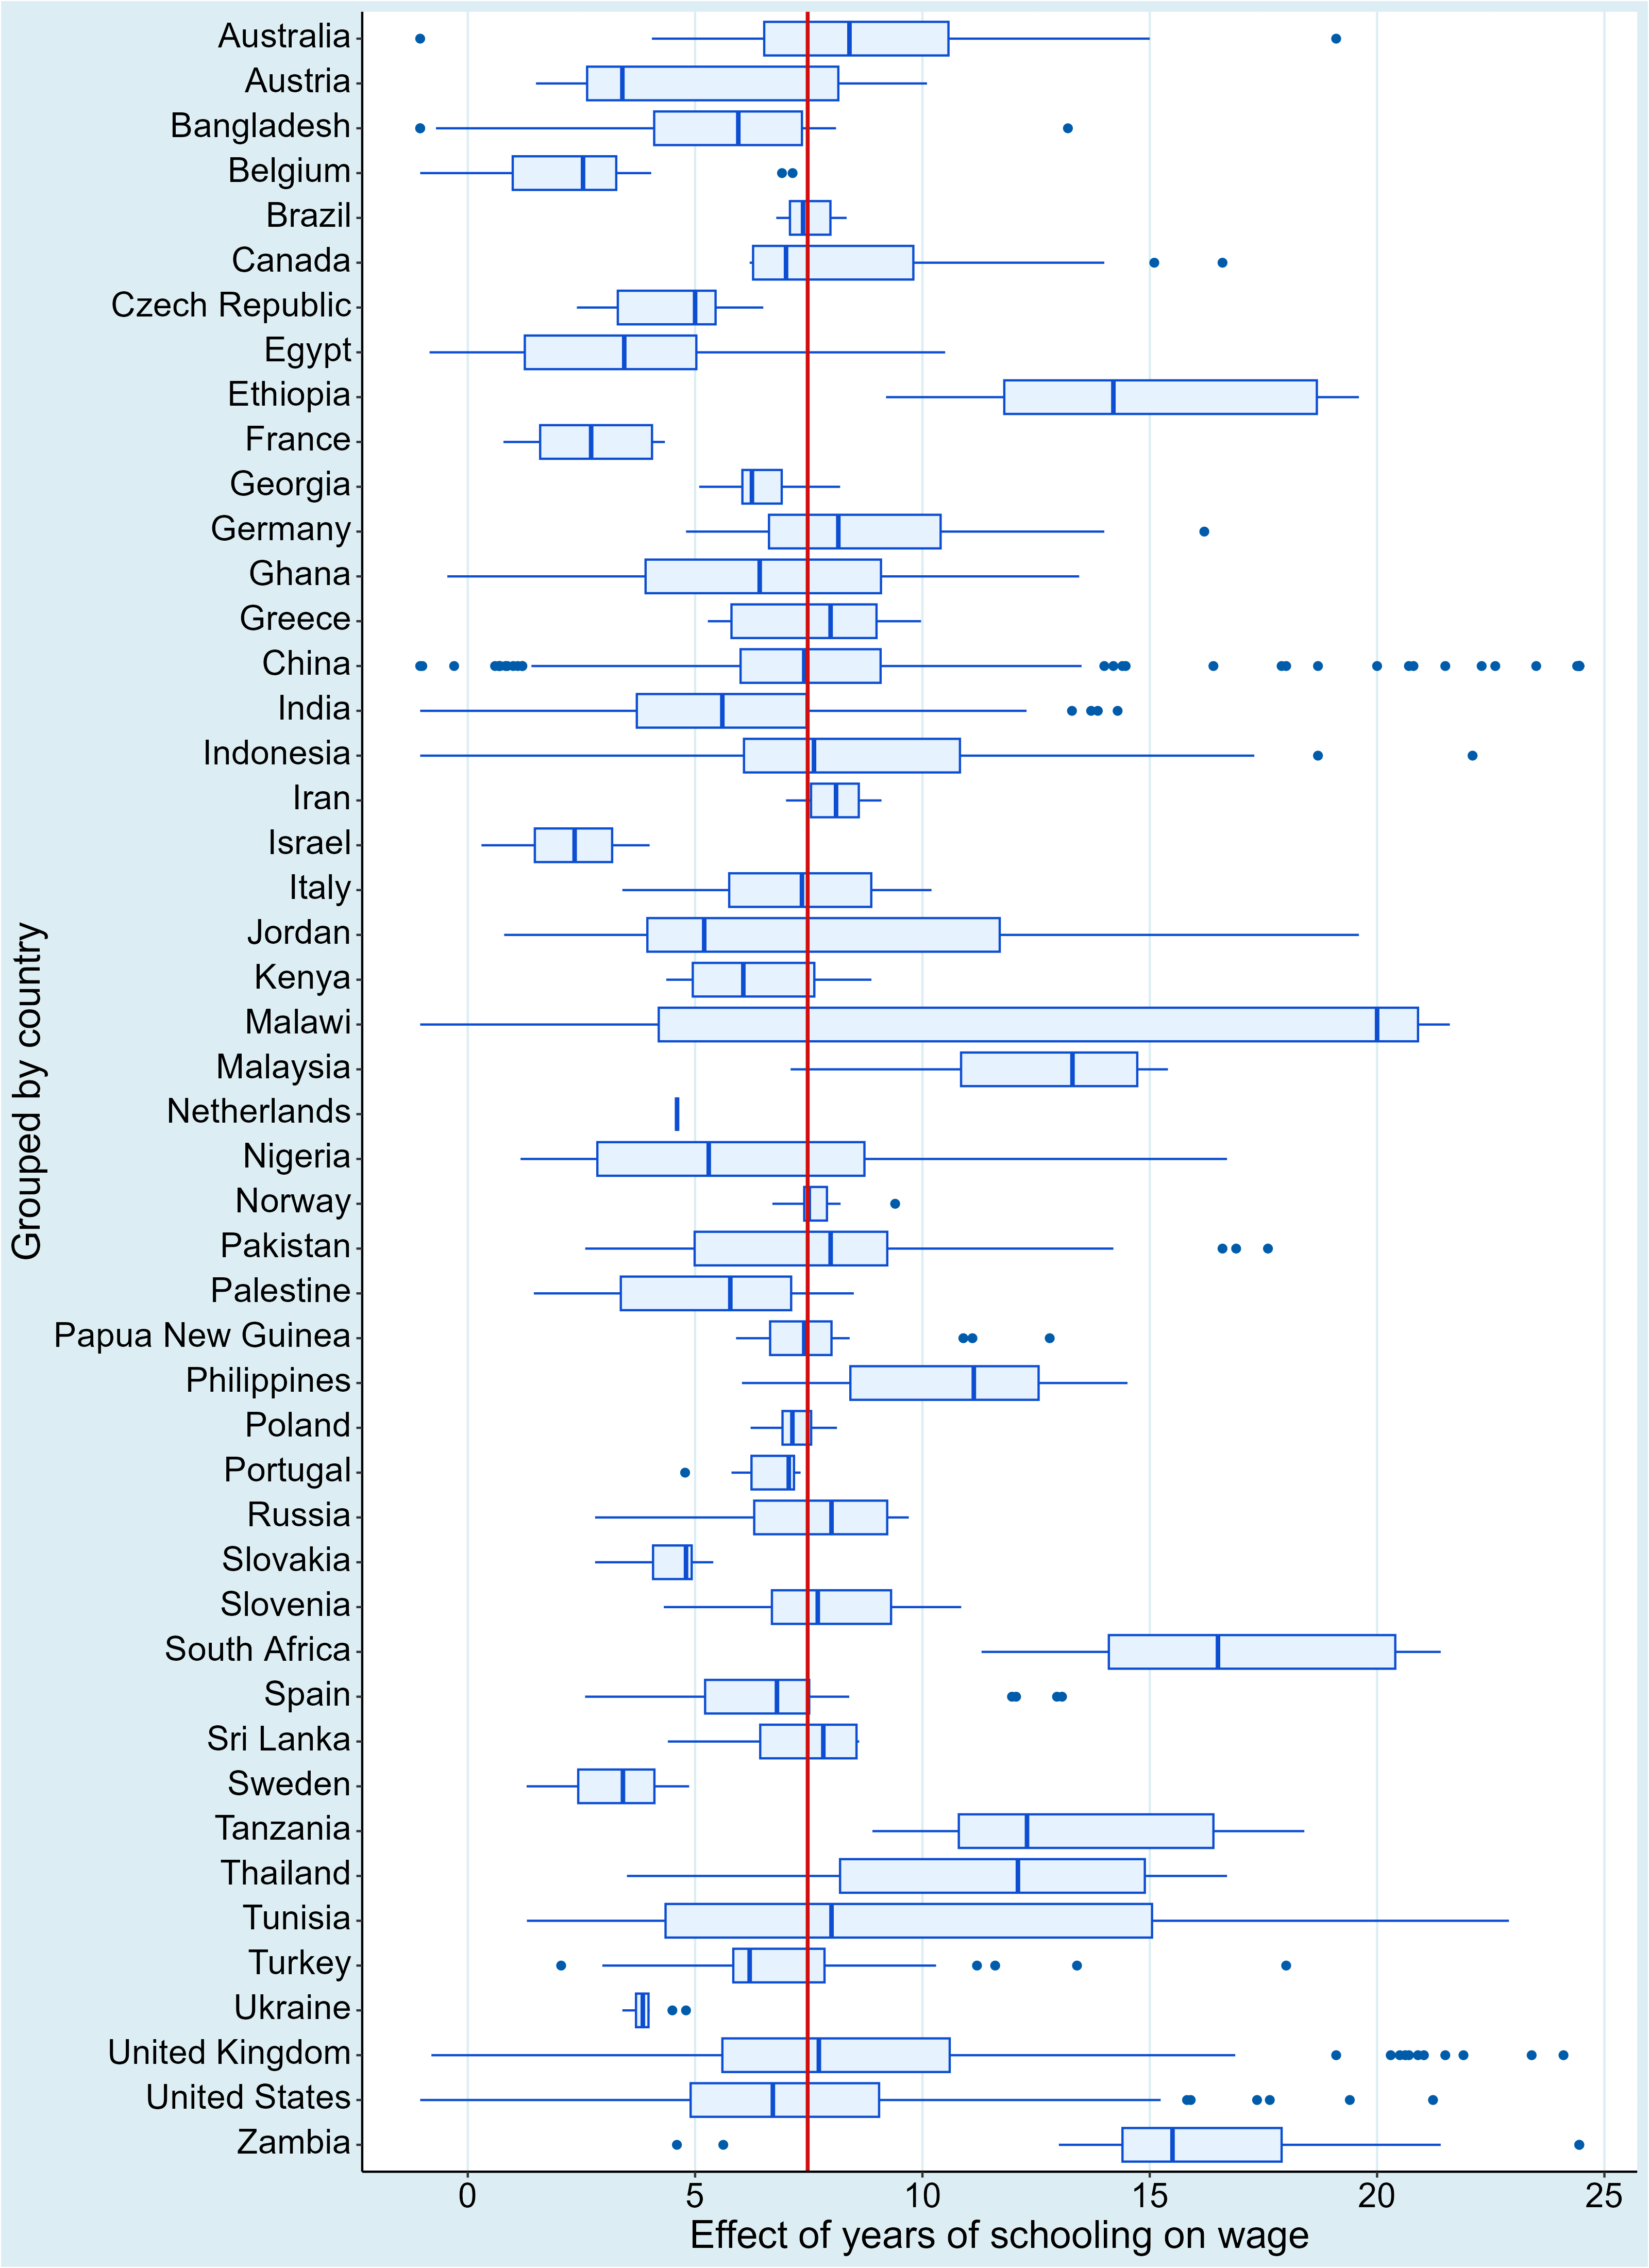
\includegraphics[width=0.9\textwidth]{Figures/box_plot_country.png}
\end{center}\vspace{-0.7cm}
\captionsetup{width=0.9\textwidth, font = scriptsize}
\caption*{\emph{Note:} This figure shows a box plot where the reported estimates are grouped at the country level. The data of all 48 countries from the data set is displayed. The red line represents the average effect across the literature. Each box's length represents the interquartile range between the 25th and 75th percentiles. The dividing line within each box indicates the median value. The whiskers extend to the highest and lowest data points within 1.5 times the range between the upper and lower quartiles. Outliers are depicted as blue dots. The data is winsorized at 1\% level.}
\end{figure}
